\section{Analysis and Results}
\label{sec:analysis}

Our pipeline ingested 600 \ac{warc} files: 300 files for responses with a successful status code and 300 files for responses with various other status codes.
The \ac{regex} \texttt{\textasciicircum.+-0000(0|1|2)\textbackslash .warc\textbackslash .gz\$} was used to select these 300 files from each data subset.
Each \ac{warc} file containing successful responses is approximately 900~MiB in size, while each file containing non-successful responses is about 29~MiB.
Thus, all compressed \ac{warc} files with successful status codes amount to approximately 264~GiB, and those with non-successful status codes to approximately 8~GiB.
The total data size fetched from Common Crawl is roughly \textbf{272~GiB}.
The total number of crawled responses ingested is \textbf{7,440,858}.

After transformations, specifically the \ac{cctld} selection, the \texttt{fact\_website} table contains \textbf{3,117,139} entries, 4,323,719 fewer than those ingested into the bronze layer.
This means that 41.9\% of all crawled websites fetched used a \ac{cctld}.

After a full pipeline run, the MinIO \ac{gui} and the \texttt{df} Linux \ac{cli} tool report 159.3~GiB of mounted storage space in use.

In the following section, we will discuss the pipeline's runtime performance.
Then, we will present the results of exemplary analyses on the ingested Common Crawl data as well as on combinations of data from different sources.


\subsection{Pipeline performance}
\label{sec:analysis-pipeline}

All Dagster assets exhibit varying execution times.
\Cref{tab:analysis-dataset-asset-times} details the durations of asset executions measured over a full pipeline run.

\begin{table}[H]
    \centering
    \begin{tabular}{|c|c|c|c|c|}
    \hline
    \textbf{Namespace} & \textbf{Type} & \textbf{Name} & \textbf{Duration} & \textbf{Configuration} \\
    \hline
    raw & seed & common\_crawl & 00:06:50 & - \\
    raw & seed & country\_codes & 00:02:01 & - \\
    raw & seed & web\_technologies & 00:02:00 & - \\
    raw & source & common\_crawl & 36:20:02 & 200responses \\
    raw & source & common\_crawl & 03:21:18 & non200responses \\
    raw & source & country\_codes & 00:00:47 & - \\
    raw & source & web\_technologies & 00:00:43 & - \\
    staging & dimension & common\_crawl & 00:04:39 & - \\
    staging & dimension & country\_codes & 00:03:02 & - \\
    staging & dimension & web\_technologies & 00:04:06 & - \\
    marts & fact & website & 02:27:29 & - \\
    - & - & charts & 00:04:47 & - \\
    \hline
    \end{tabular}
    \caption{Asset execution times.}
    \label{tab:analysis-dataset-asset-times}
\end{table}

The larger \texttt{common\_crawl} seed (2.7~MB) takes almost seven minutes to load, while the smaller \texttt{country\_codes} and \texttt{web\_technologies} seeds (below 15~kB each) take around two minutes to load.
Loading these smaller seeds takes longer than expected, given that large volumes of data can be processed relatively quickly; if it is possible to download, decompress, process, compress, and persist over 250~GiB of data within 36 hours using the \texttt{common\_crawl} asset, a local \ac{csv} file of 2.7~MB should theoretically load in under a second.

Closer inspection of the dbt seed run reveals that the majority of time is consumed by dbt's startup (one minute), processing (half a minute for small files, four minutes for larger files), and shutdown (an additional half minute).

The exact cause of these long durations remains uncertain, though debug information indicates that most of the time is spent after \texttt{Close} commands on Spark connections are logged.
This delay does not occur when using a \texttt{session} connection instead of a \texttt{thrift} connection in dbt's profiles configuration, as shown in \cref{lst:implementation-pipeline-transformation-dbt-profiles}.
However, using a \texttt{session} connection can cause issues in PySpark's \ac{sql} statements due to unescaped characters within the seed sources, such as carets.

Further research indicates that dbt, in conjunction with its Spark adapter, initially builds a cache of all schema and table metadata.
dbt attempts to execute a \texttt{SHOW TABLE EXTENDED} \ac{sql} command, which is unsupported in Spark's Data Source V2 \ac{api} in versions prior to Spark \texttt{4}\footnote{Spark \texttt{4} is not yet released at the time of writing, although a preview was released on 2024-09-26.}.
Consequently, dbt falls back on \texttt{SHOW TABLE} and \texttt{DESCRIBE TABLE} statements, which become increasingly time-consuming as the number of schemas and tables grows.

Sourcing a table from an \ac{html} page and \ac{json} files from GitHub, as done for country codes and web technologies respectively, takes around 40 seconds.
Most of that time passes while the Spark session initializes.

Each test run by dbt requires about 20 seconds to complete.
For \texttt{dimension\_common\_crawl}, this results in a total of 2:19 minutes for seven checks.
The same checks take five to ten seconds on a cold PySpark session and under two seconds on a warm PySpark session\footnote{A cold session is one that has not run any queries since startup, whereas a warm session has already run a query.}.

Materializing the \texttt{website} fact table takes about 2.5~h, which is more than 14 times faster than the ingestion of Common Crawl data alone.
This demonstrates that operations on data stored within local table structures are highly efficient with respect to performance, even when running more complex \texttt{JOIN} operations and extensive \ac{regex} pattern matching.

Finally, the 17 \ac{px} charts materialize in under five minutes.
While most generated chart files have a size of approximately 5~MB, some include data points for all table rows, resulting in file sizes between 50~MB and 100~MB.
If more data is added to these tables, the chart generation strategy for those large chart files would need to change.
Even now, opening these large chart files locally in a modern browser on an ordinary computer takes more than ten seconds.

A typical log output of a Dagster asset's function run, including time measurements, is shown in \cref{lst:appendix-listings-spark-logs}.
The time measurements stem from the decorator defined in \cref{lst:dagster-utility-performance-measurement} for performance assessment.
This log output shows sub-second durations for data stream fetching (lines 1, 2, and 4).

From lines 6 to 24, the log shows Spark initializing with the \ac{jar} files required for Iceberg table format support on S3 object storage.
The following lines display the Spark job running.
The warnings can be ignored, as we do not want to eliminate website \ac{html} payloads above 1000~KiB from our dataset and splitting the \ac{html} would not be trivial.
The first write execution (68.0258~s, line 26) always takes longer than subsequent writes (e.g., 42.6831~s, line 28).
Write times would be considerably less if we simply appended data, without removing duplicates first.


\subsection{Dataset analysis}
\label{sec:analysis-dataset}

The following figures visualize key metrics of our dataset.
The figures are generated using \ac{px} in functions such as the one shown in \cref{lst:implementation-pipeline-visualization-chart}.

All charts in this thesis are images of \ac{html} documents that allow interactivity, such as hovering over fields to show details, clicking on legend elements to hide respective fields, and zooming in and out of graph areas.
The first figure, \cref{fig:analysis-dataset-chart_source_charset_pie}, shows a mouse hovering over a field as an example of interactivity; all subsequent graphs are shown without such overlays.

We first inspect the bronze layer's Common Crawl dataset as ingested by the methods outlined in \cref{sec:implementation-pipeline-ingestion}.
This step is important as it allows us to validate the source data quality.
On this basis, we then proceed with a more detailed analysis of country-specific web technology usage as envisioned in \cref{sec:design-envisioned-result}.


\subsubsection{Analysis of source data}
\label{sec:analysis-dataset-source}

After the ingestion of all 600 \ac{warc} files, the silver layer's staging view was materialized, and one of its checks failed.
This test failure was due to only two entries out of more than seven million, which had status codes of \texttt{706} and \texttt{999}.
We defined a custom macro in \texttt{dbt}, as shown in \cref{lst:implementation-pipeline-transformation-dbt-macro}, that allowed us to catch unexpected data.

At the time of writing, the pages that returned the implausible status codes to Common Crawl now return the expected status code of \texttt{200} to a standard browser request.
The web servers may be configured to respond differently to requests originating from Common Crawl, either due to a technical flaw or intentionally.

These outlier status codes were caught by coincidence, thanks to our previous exemplary test definition.
A guess-based approach for testing would be inefficient to continue, which is why we examine data distributions in the following graphs.
We aim to use visual representations to gain insights into the quality of our data.

The data source provider, Common Crawl, also offers statistics on their dataset, as referenced in \cref{sec:related-work-big-data-datasets}.
This allows for comparisons between the full dataset, as analyzed by Common Crawl, and our subset of it, which will be discussed in the following chapter, \cref{sec:evaluation}.

The first metric we inspect is the \ac{http} charset distribution, i.e., a distribution of character encodings that map page contents' bytes to their text representation.
As displayed in \cref{fig:analysis-dataset-chart_source_charset_pie}, the vast majority (87.6\%) of \ac{http} responses specify \texttt{utf-8} as charset, representing 6,516,178 pages.
The next most commonly specified charset is not \texttt{iso-8859-1}, as might be expected if a charset were mandatory, but an empty charset specification (8.72\%).
\texttt{iso-8859-1}, also known by its \href{https://home.unicode.org/}{\textit{Unicode}} block name \textit{Latin-1}, is a single-byte encoding as opposed to \texttt{utf-8}'s multibyte encoding and ranks third (2.51\%).
For readability, we group all charsets with a frequency below 0.1\% into a category named \texttt{Other}, which comprises around 0.7\% of all charset specifications.

\begin{figure}[H]
    \centering
    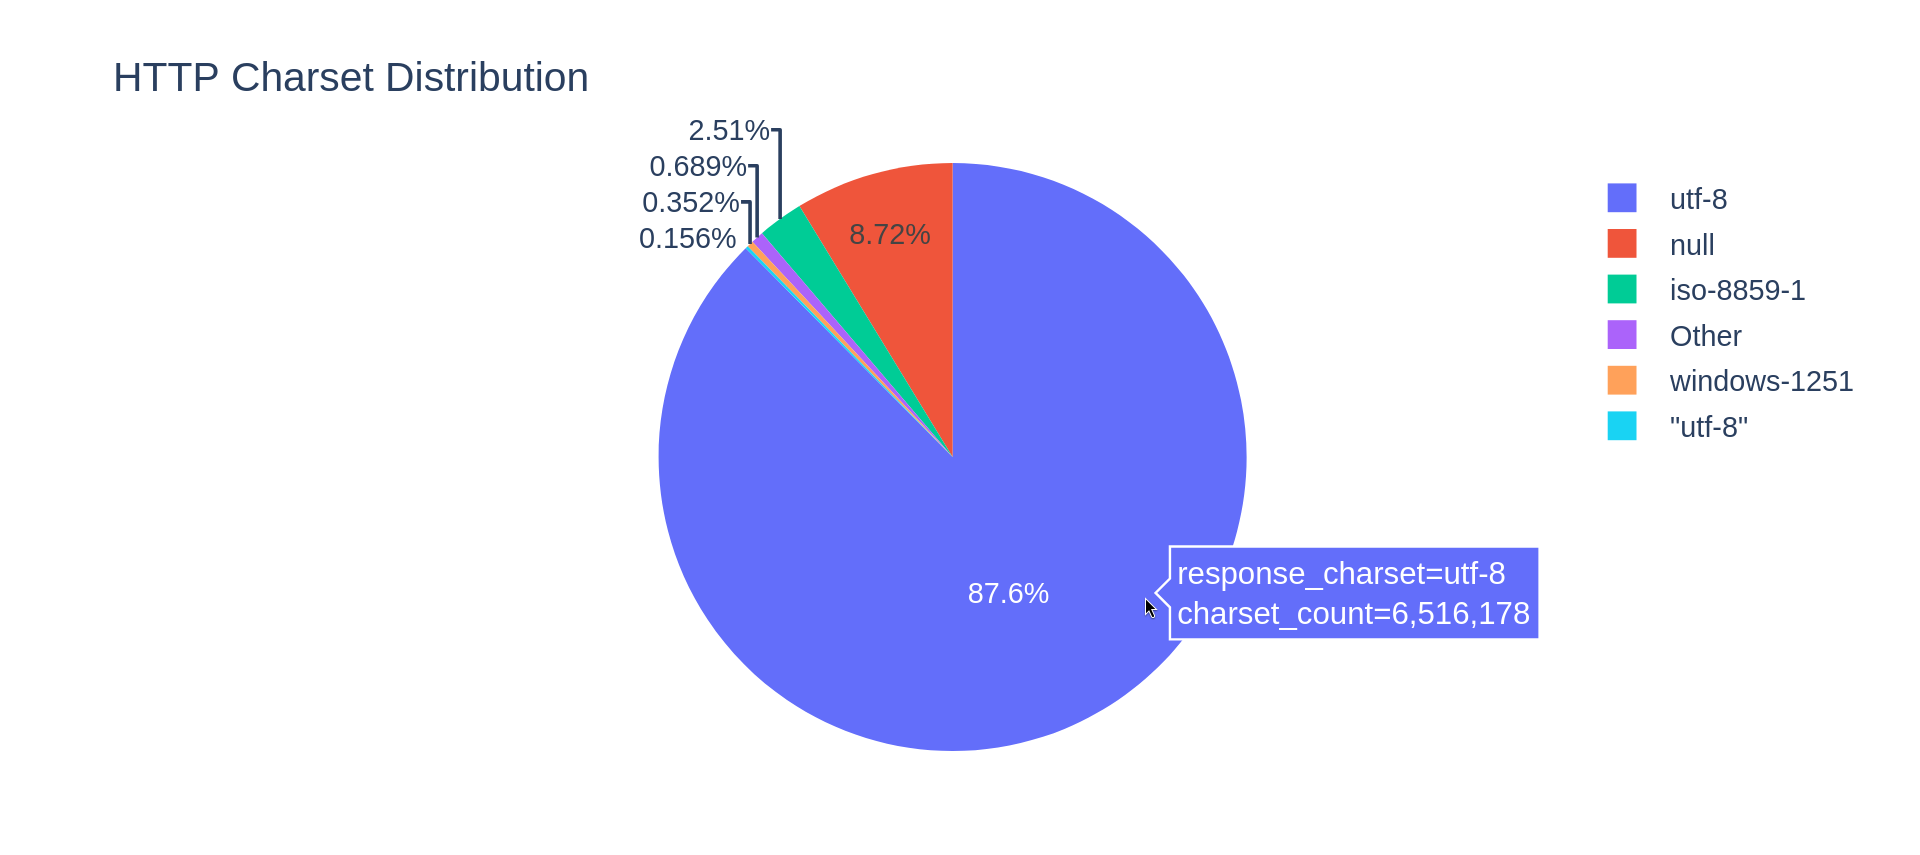
\includegraphics[width=\textwidth]{figures/charts/large/chart_source_charset_pie.png}
    \caption{Charset distribution with hover overlay.}
    \label{fig:analysis-dataset-chart_source_charset_pie}
\end{figure}

\Cref{fig:analysis-dataset-chart_source_charset_pie} already provides an important insight into data quality: the fourth most common charset among all responses with a specified charset is \texttt{"utf-8"} (i.e., \texttt{utf-8} with quotation marks).
While this formatting is likely not compliant with specifications, it may go undetected by web developers as clients could work around such common misconfigurations.
However, this hypothesis has not been researched further.

If future research shows such client workarounds to be common, a possible data quality improvement could be to remove quotation marks in the view definition set in \cref{lst:implementation-pipeline-transformation-dbt-model} so that quoted variants are not counted separately.
A second reason supporting this improvement could be that modern browsers fall back to \texttt{utf-8} when encountering an unexpected charset, such as one with quotes.

To explore the distribution of charsets besides \texttt{utf-8} and \texttt{null}, we exclude these most common encodings and obtain the graph shown in \cref{fig:analysis-dataset-chart_source_charset_pie_excluding_utf8}.
In this graph, all charsets that appear in less than 0.8\% of the remaining cases, i.e. less than 0.03\% of all ingested websites, are grouped into the \texttt{Other} category.
Besides the quoted variant of \texttt{utf-8}, another variant specified as \texttt{utf8} is now visible, occurring in 3,803 of the ingested websites (0.05\%).

\begin{figure}[H]
    \centering
    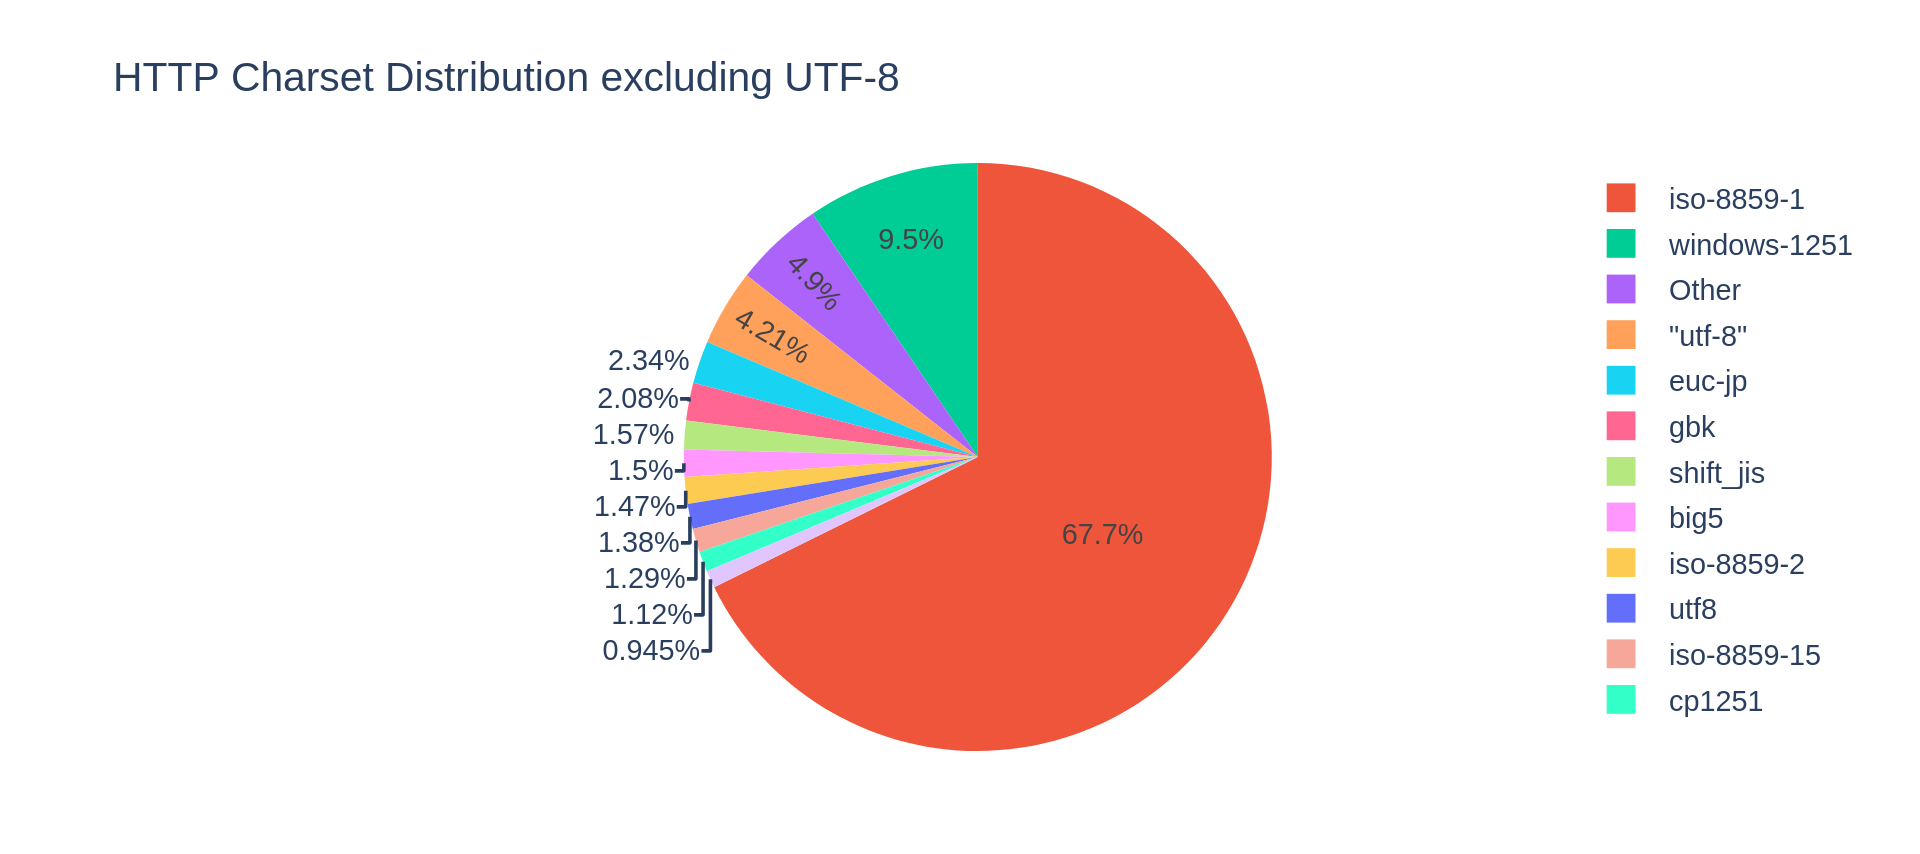
\includegraphics[width=\textwidth]{figures/charts/large/chart_source_charset_pie_excluding_utf8.png}
    \caption{Charset distribution, excluding \texttt{UTF-8}.}
    \label{fig:analysis-dataset-chart_source_charset_pie_excluding_utf8}
\end{figure}

Now that we are aware of the various charsets in use, we analyze website size next, as a website's size depends on the amount of content and, to some extent, on the charset used.

\Cref{fig:analysis-dataset-chart_source_payload_size_bar_count} shows the distribution of \ac{http} payload size ranges.
There are 2.9~million websites with a payload size of zero to 50~kB and about half as many in each successive 50~kB range, except for websites in the 1~MB to 1.05~MB range.
Since the graph does not show websites larger than 1.05~MB, it appears that there is a size limit for each website in the Common Crawl dataset of 1~MiB.

The 1~MB to 1.05~MB range stands out as the only range with a higher count of websites than any of the ranges of smaller payload size.
Presumably, there might be a technical reason that limits website payloads surpassing the 1~MiB boundary, so they appear as 1~MiB in size, though intended to be larger.
There are 138 thousand pages in our dataset that fall in the 1~MB to 1.05~MB range, while only 14 thousand pages fall in the adjacent 0.95~MB to 1~MB range.

\begin{figure}[H]
    \centering
    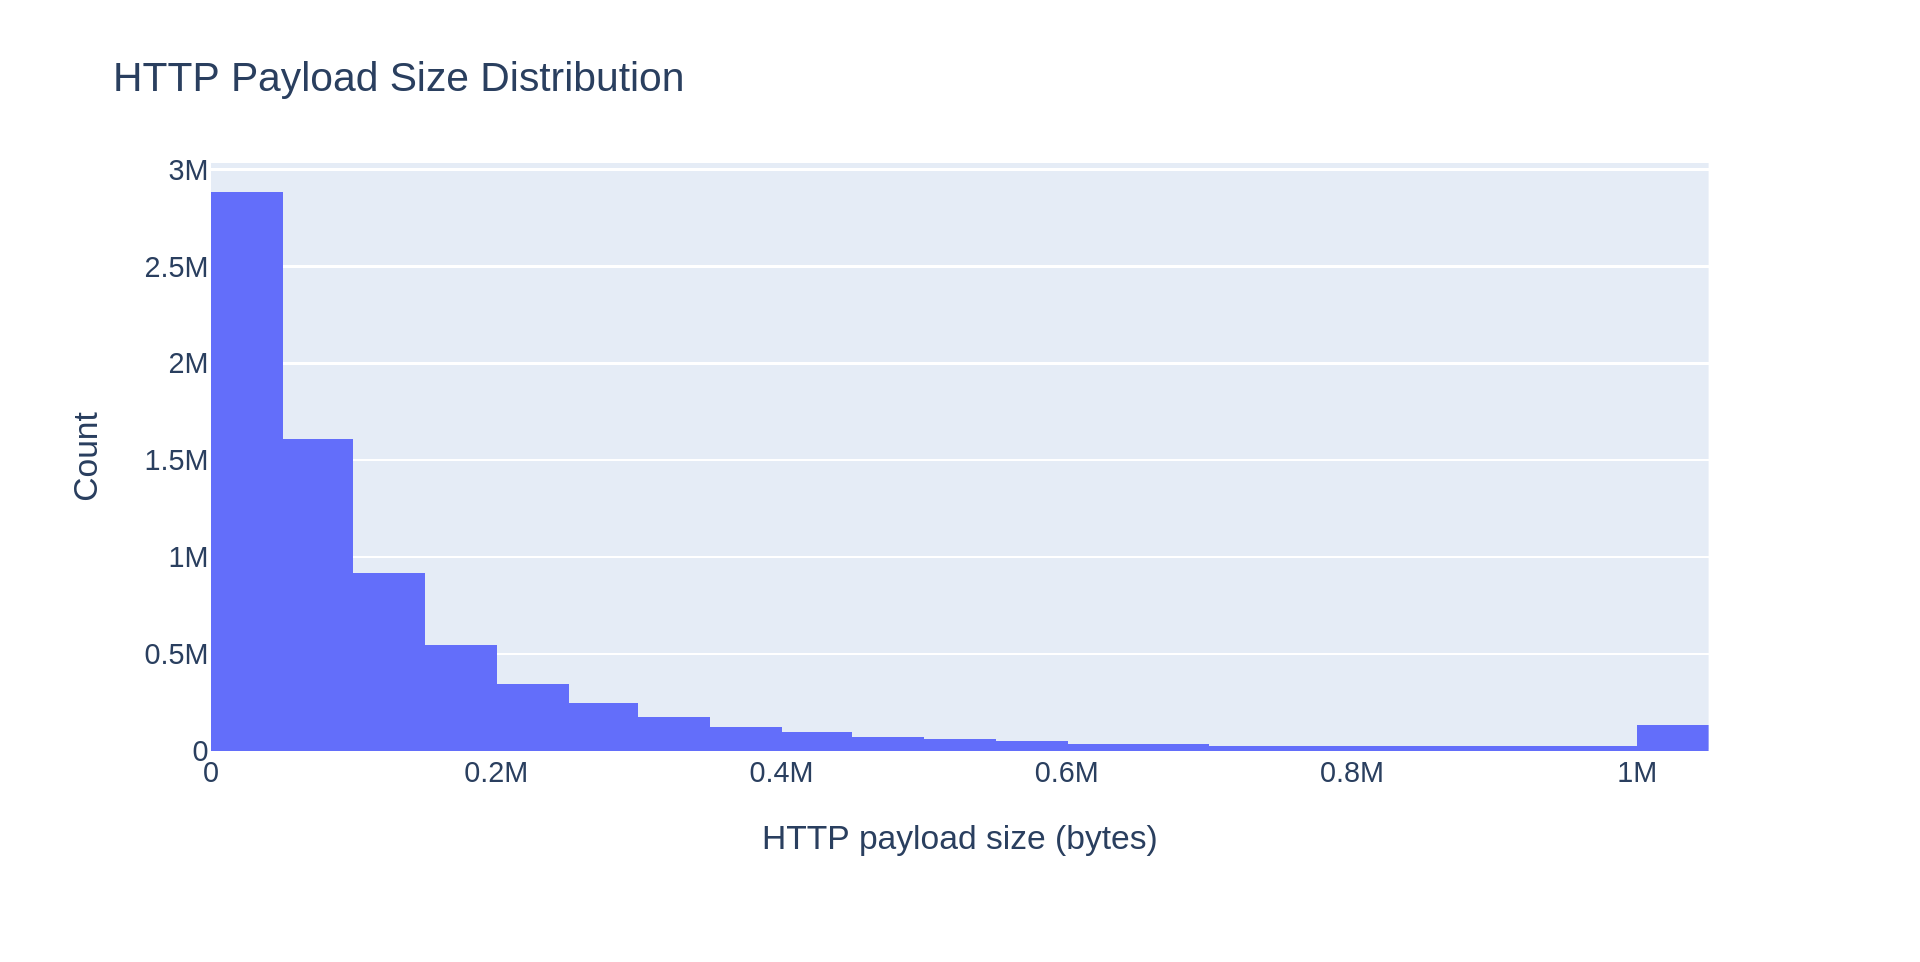
\includegraphics[width=\textwidth]{figures/charts/large/chart_source_payload_size_bar_count.png}
    \caption{Payload size distribution.}
    \label{fig:analysis-dataset-chart_source_payload_size_bar_count}
\end{figure}

A scatter plot provides another perspective on the correlation between the byte size and decoded character length of a website.
\Cref{fig:analysis-dataset-chart_source_payload_size_scatter_payload_length} shows this correlation.
Beyond the intuitive observation that no website has fewer characters than bytes, there is a notable variance in the relationship between bytes transmitted and decoded character length.

While single-byte encodings, such as \texttt{ascii} or \texttt{iso-8859-1}, appear only along the diagonal with a slope factor of one, multi-byte encodings allow multiple transmitted bytes to represent a single character.
However, there is no distinct secondary axis with a different slope factor visible in the graph, which would indicate that a charset requires a fixed byte count for each character.
Instead, multibyte character encodings appear to allow one-to-one mappings between a byte and a character as well as many-to-one mappings of multiple bytes to a character.
Furthermore, there seems to be an upper limit within the detected charsets for the number of bytes that can be decoded into a single character, apparent from the empty area in the top left.
Additionally, a horizontal line of dots can be seen at the 1~MiB payload size level, which we already observed in \cref{fig:analysis-dataset-chart_source_payload_size_bar_count}.

Regarding data quality and interpretation accuracy, it is essential to consider the representativeness of each part of the dataset inspected.
For example, \cref{fig:analysis-dataset-chart_source_payload_size_bar_count} shows that websites with smaller payload sizes are more common than websites with larger payload sizes.
This pattern is reflected in the higher density of dots in the lower left area of the graph behind \cref{fig:analysis-dataset-chart_source_payload_size_scatter_payload_length}.
Without considering this context, one might erroneously conclude that less common charsets are specified more frequently by smaller websites, as more dots with colors other than the color for the \texttt{utf-8} charset are visible in the lower left corner.
A different chart, potentially normalizing by charset frequency, would be useful to analyze the average payload size for each charset.

\begin{figure}[H]
    \centering
    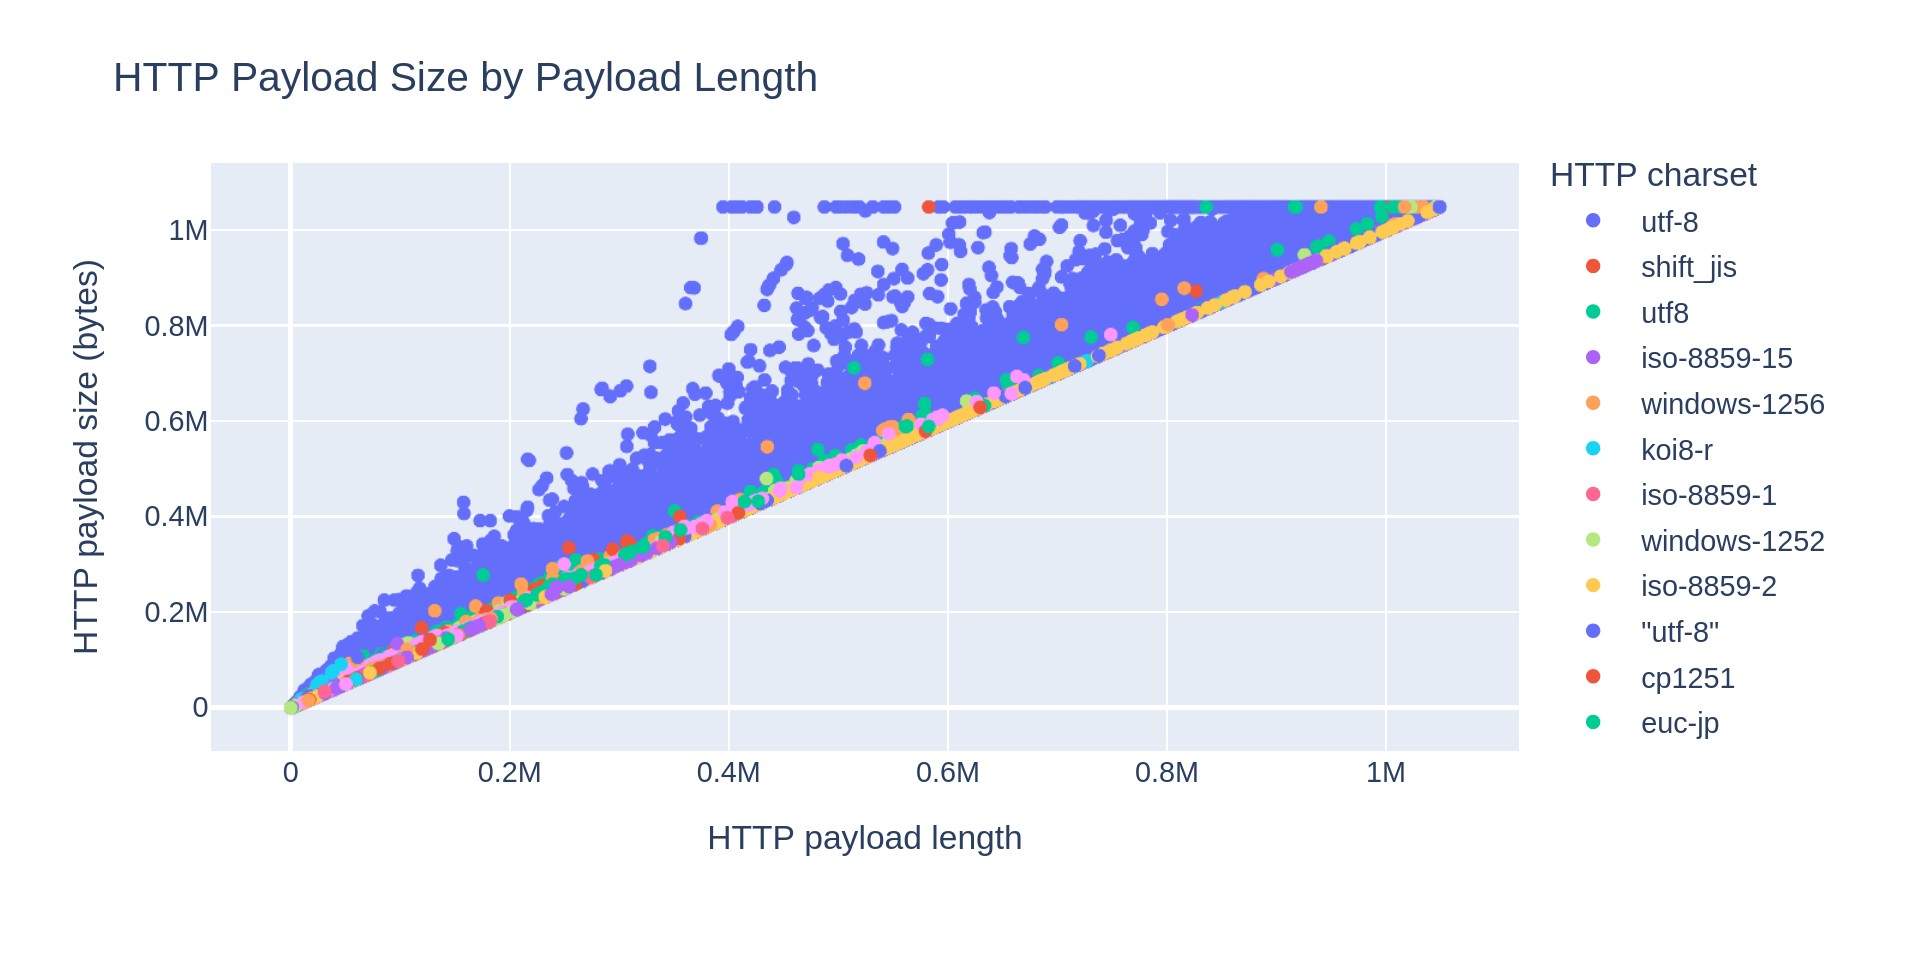
\includegraphics[width=\textwidth]{figures/charts/large/chart_source_payload_size_scatter_payload_length.png}
    \caption{Payload size by payload length.}
    \label{fig:analysis-dataset-chart_source_payload_size_scatter_payload_length}
\end{figure}

\Cref{fig:analysis-dataset-chart_source_charset_bar_payload_size} is one such chart, though without any normalization.
It shows that the average payload size of websites specifying the \texttt{"utf-8"} charset is 205~kB, while websites specifying the \texttt{cp950} charset have an average payload size of 116~B.
Websites specifying \texttt{latin} as a charset even have an average size of zero, meaning they returned only headers but no \ac{html} body.

However, this chart is also limited in expressiveness, as the averages shown are more meaningful for frequently used charsets.
For example, a charset that is only used by one page of 0.5~MB, perhaps due to a typo like \texttt{utf -8} (sic!), would set the average for that invalid charset to 0.5~MB, making it the highest in our measurements.
Considering this, the high average payload size for charset \texttt{"utf-8"} is notable, as \cref{fig:analysis-dataset-chart_source_charset_pie_excluding_utf8} shows that this charset is one of the most common in our dataset (2.51\%) and therefore possesses meaningful representativeness.

Our dataset includes both successful and non-successful responses, so a bar chart similar to \cref{fig:analysis-dataset-chart_source_charset_bar_payload_size} can be created for average payload sizes and \ac{http} status codes instead of charsets, as shown in \cref{fig:analysis-dataset-chart_source_response_code_bar_payload_size}.
As before, a status code like \texttt{706}, returned by only one website, could appear as the highest average if that website were particularly large.
However, this is not the case: the most common response status code is \texttt{200} (85\%), followed by code \texttt{301} (5.97\%) and \texttt{404} (4.95\%), as shown in \cref{fig:analysis-dataset-chart_source_response_code_pie}.
For these codes, the averages in \cref{fig:analysis-dataset-chart_source_response_code_bar_payload_size} are most meaningful.

Websites returning a successful response have an average payload size of 159~kB; for code \texttt{301}, the average payload size is 1.9~kB, and for websites returning a \texttt{404} error, the average payload size is 89~kB.
The low payload size for code \texttt{301} makes sense, as such responses indicate a permanent redirect, so browsers likely do not render these websites.

\begin{figure}[H]
    \centering
    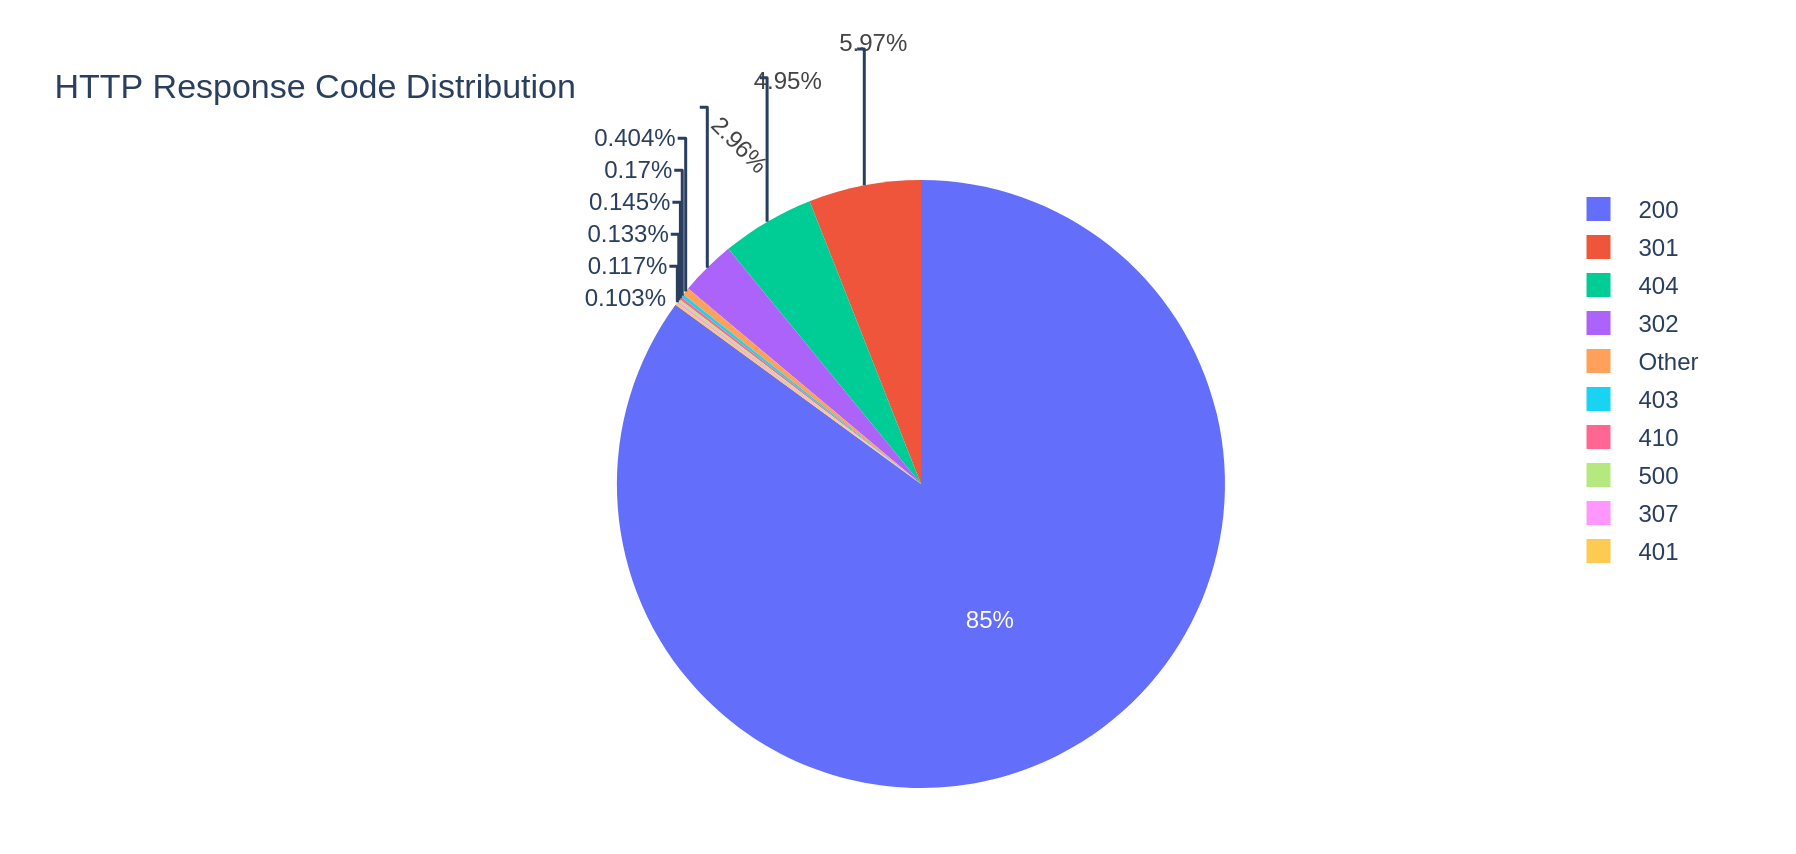
\includegraphics[width=\textwidth]{figures/charts/large/appendix/chart_source_response_code_pie.png}
    \caption{Response code distribution.}
    \label{fig:analysis-dataset-chart_source_response_code_pie}
\end{figure}

\Cref{fig:analysis-dataset-chart_source_charset_heatmap_response_code} compares charsets and response codes directly.
The heatmap displays a high frequency of status code occurrences per charset in yellow, with a low count shown in purple.
According to \ac{rfc} 7231, the \texttt{200} to \texttt{299} range is designated for successful responses, the \texttt{300} to \texttt{399} range for redirections, the \texttt{400} to \texttt{499} range for client errors, and the \texttt{500} to \texttt{599} range for server errors.

This chart also suffers from representation issues, such as with the \texttt{latin} charset, which is represented by only one website in our dataset.
For the \texttt{latin} charset, the \texttt{300} to \texttt{399} range shows up in bright yellow, as the single website returned a \texttt{302} response.
The chart is normalized by total charset count so that fields for charsets other than \texttt{utf-8} still exhibit color variation.

Incorrectly formatted charsets are prevalent, and 85\% of all responses have the \texttt{200} status code.
Due to these facts, additional comparisons among frequently occurring charsets would be necessary to identify patterns, such as whether certain charsets are more often associated with error pages than with successful responses.


\subsubsection{Analysis of aggregate data}
\label{sec:analysis-dataset-aggregate}

Now that we have established sufficient context to estimate the quality of our source data, we can shift our focus to analyses of global semantics.
More specifically, we will inspect web technology usage on both global and country-specific scales.
The graphs shown in this section are based on queries against the \texttt{fact\_website} table from the gold stage's \texttt{marts} namespace.

First, we visualize the mapping of \acp{cctld} to countries, which required assigning a matching ISO 3166 alpha-3 code to each \ac{uri}, as shown in \cref{lst:implementation-pipeline-visualization-chart}.
\Cref{fig:analysis-dataset-chart_fact_uri_choropleth} displays a choropleth map on which countries appear more yellow the more \acp{uri} with a matching \ac{cctld} they have, and more purple if they have fewer \acp{uri} with a matching \ac{cctld}.

Immediately, the country with the largest landmass, Russia, stands out in bright yellow.
There are approximately 326,177 websites with a \texttt{.ru} \ac{tld} in our dataset, accounting for 10.5\% of all websites with a \ac{cctld} and 4.4\% of all websites ingested overall.
Next, Germany, with its \ac{cctld} \texttt{.de}, is marked in light green as another country with a significant share of websites: approximately 287,434 websites, representing 9.2\% of the \ac{cctld} subset and 3.9\% of all ingested websites, are attributed to Germany.
Countries attributed with between 100,000 and 200,000 websites include the United Kingdom (159,216), Japan (154,911), Italy (140,071), France (132,077), Poland (124,659), Brazil (116,443), and the Netherlands (112,973).
Countries with between 50,000 and 100,000 websites include Australia (80,816), Czechia (77,221), Spain (69,634), Canada (68,759), China (57,013), and Ukraine (50,415).
All countries in Africa appear in purple, indicating that only a few websites are assigned to African \acp{cctld}.

\begin{figure}[H]
    \centering
    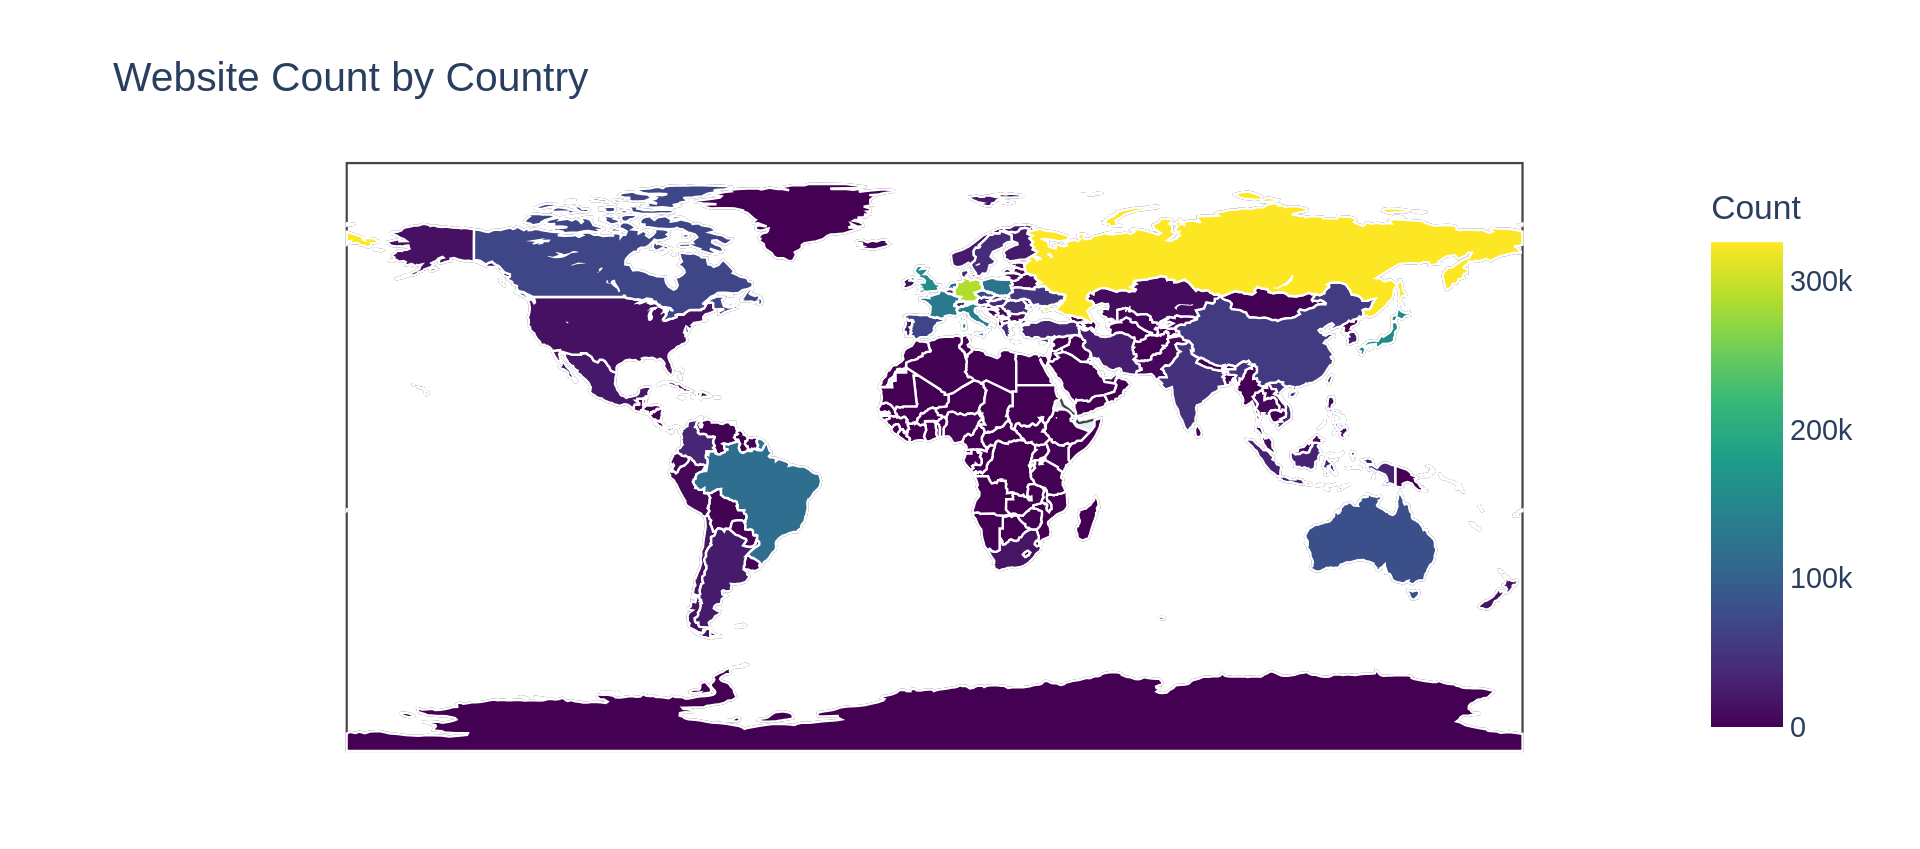
\includegraphics[width=\textwidth]{figures/charts/large/chart_fact_uri_choropleth.png}
    \caption{Total website count by country.}
    \label{fig:analysis-dataset-chart_fact_uri_choropleth}
\end{figure}

Comparing \cref{fig:analysis-dataset-chart_fact_uri_choropleth} with a choropleth map of world population in \cref{fig:analysis-dataset-population} reveals several differences.
The two most populous countries, India and China, each with over 1.4 billion people, rank far below Russia in website count within our dataset.
Although Russia has a relatively high population of 145 million, it is still only about one-tenth of the population of India or China.
Europe and South America display similar patterns on both maps.
In North America, however, the roles of Canada and the United States appear reversed: while the U.S. population (345 million) is nearly ten times that of Canada (40 million), Canada has about four times as many websites (60,000) as the U.S. (15,000) in our dataset.
Similarly, African countries exhibit much greater variation in population counts compared to their website counts~\cite{WPR2024}.

It is also important to note that \cref{fig:analysis-dataset-population} uses a different color scale, not only in terms of color range but also with an exponential increase in saturation, whereas \cref{fig:analysis-dataset-chart_fact_uri_choropleth} employs a continuous color scale.

\begin{figure}[H]
    \centering
    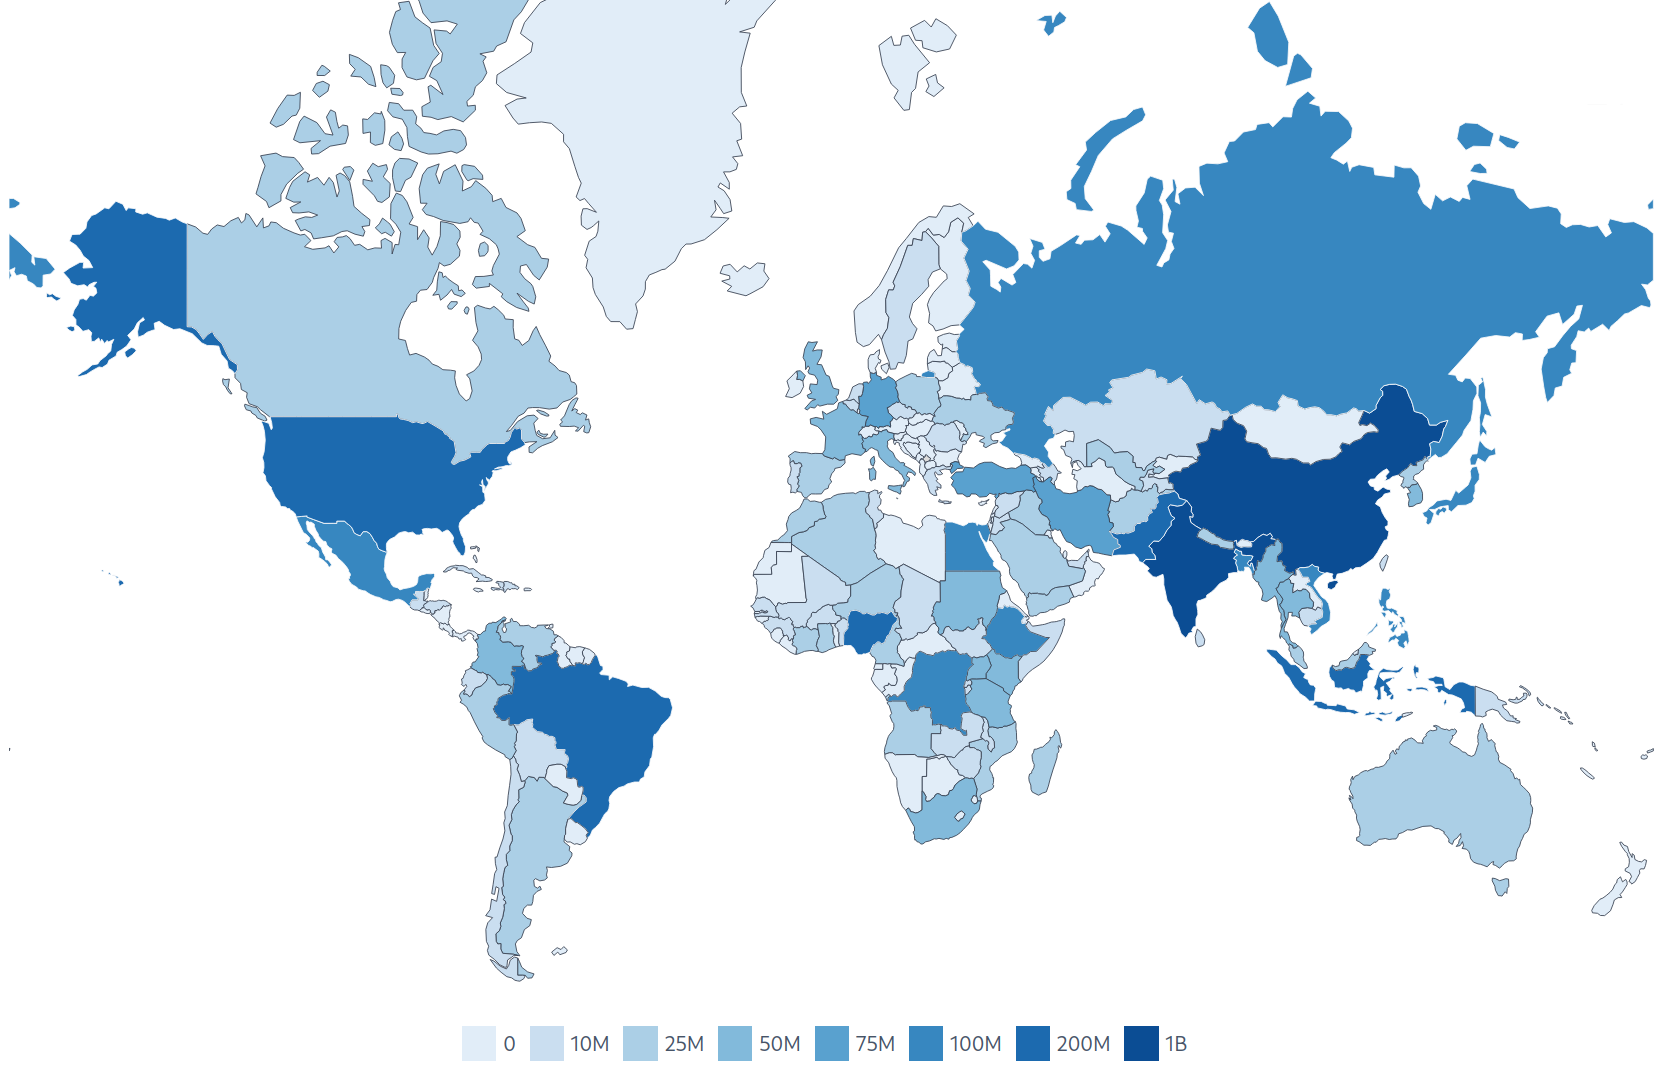
\includegraphics[width=0.6\textwidth]{figures/charts/population_choropleth.png}
    \caption{Total Population by Country, 2024~\cite{WPR2024}.}
    \label{fig:analysis-dataset-population}
\end{figure}

All 3,117,139 \ac{html} sources were pattern-matched using 422 \acp{regex} to determine indicators of specific web technology usage.
In total, 3,779 web technologies were sourced from Wappalyzer, of which 325 had defined \acp{regex} for matching on \ac{html} such as \texttt{\textless img[{\textasciicircum}>]+moodlelogo} for \href{https://moodle.de/}{\textit{Moodle}}.
Some web technology definitions had multiple \acp{regex} assigned.

The most frequently detected web technology across all \ac{html} sources is WordPress, identified in 924,000 \ac{html} sources, equivalent to 36.6\% of all web technology detections.
The second most frequently detected technology is \textit{Google Tag Manager}, with 552,000 detections, accounting for 21.9\% of all detections.
The remaining technologies in this ranking each have fewer than 90,000 detections: \textit{Gravatar} (89,000), \textit{YouTube} (89,000), and \textit{LiveInternet} (84,000).
Ten web technologies were detected on only one page, including \textit{SonarQube}, \textit{cPanel}, and \textit{Microsoft Publisher}.
\Cref{fig:analysis-dataset-chart_fact_web_technology_bar_top_10} shows the top 10 ranking web technology detections, and \cref{fig:analysis-dataset-chart_fact_web_technology_pie} represents similar information in a pie chart.

\begin{figure}[H]
    \centering
    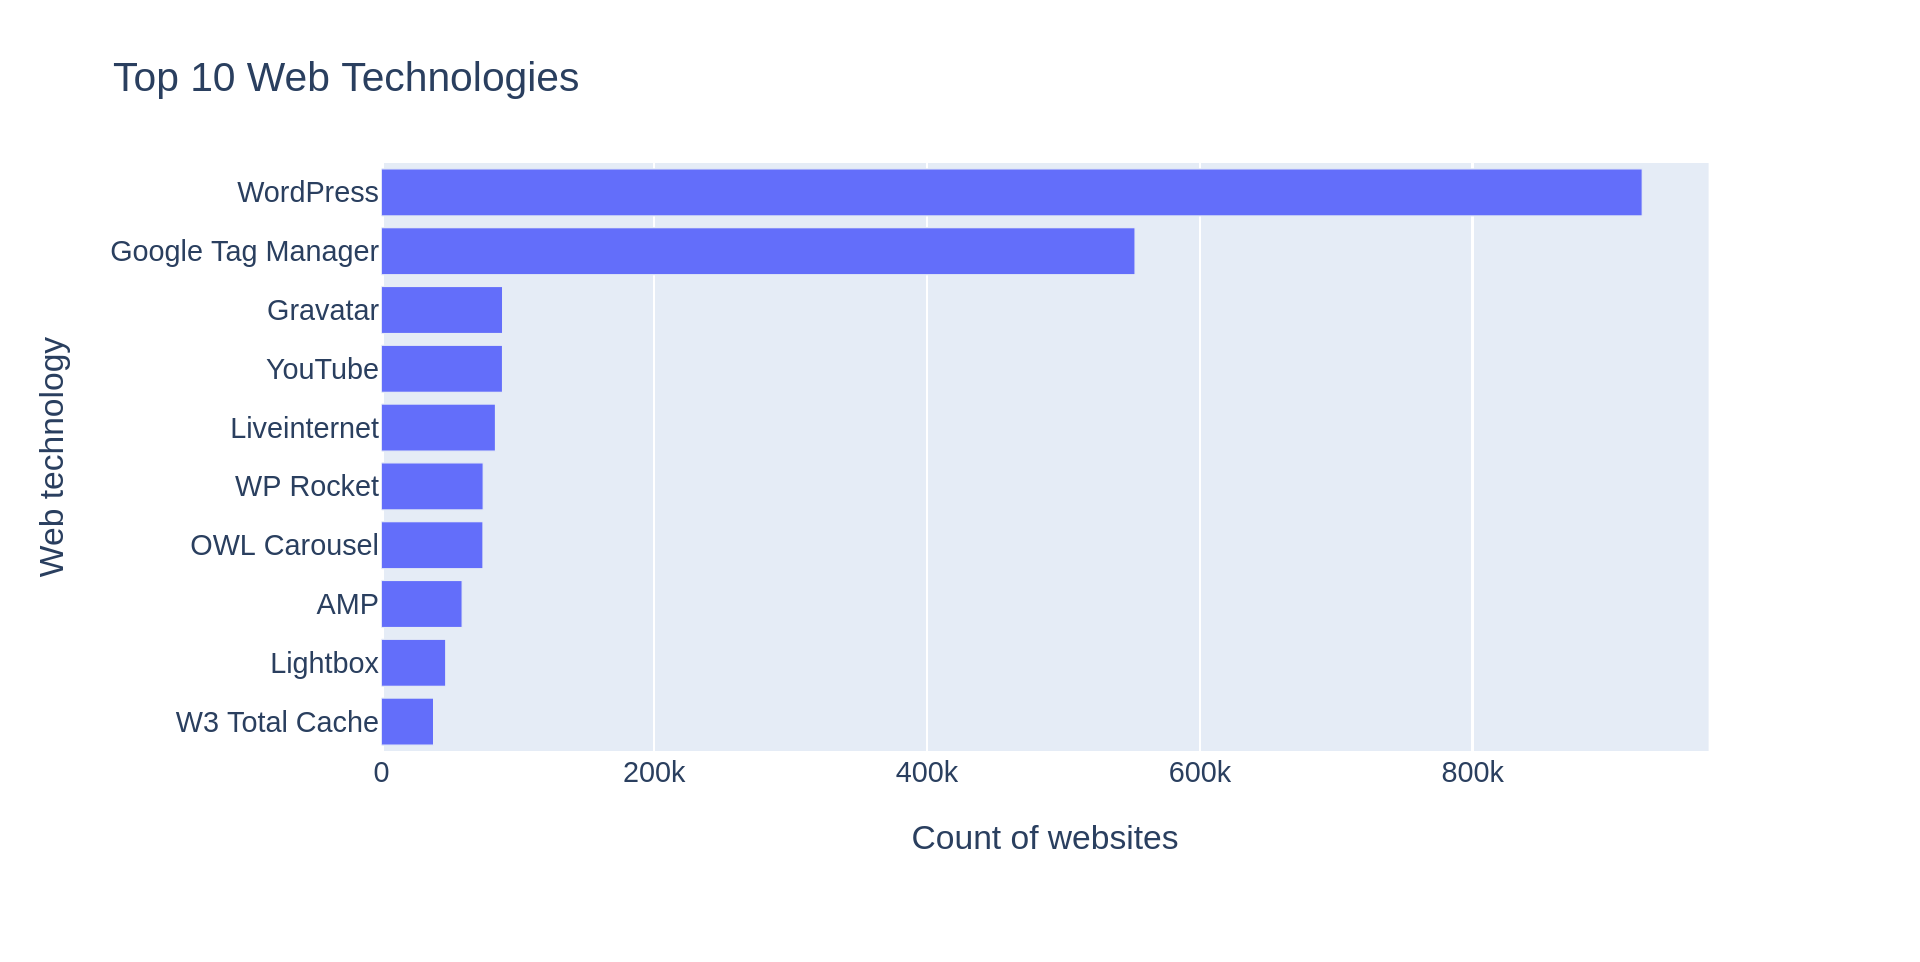
\includegraphics[width=\textwidth]{figures/charts/large/chart_fact_web_technology_bar_top_10.png}
    \caption{Top 10 web technologies found.}
    \label{fig:analysis-dataset-chart_fact_web_technology_bar_top_10}
\end{figure}

Next, we combine web technology detections with country information in \cref{fig:analysis-dataset-chart_fact_web_technology_choropleth_average}.
This choropleth map shows the average count of web technologies on websites for each country.
Due to the limited expressiveness of data from countries with relatively few attributed websites, we focus on the countries previously discussed for \cref{fig:analysis-dataset-chart_fact_uri_choropleth} and omit discussion of color variation in Africa.

The countries with the highest number of attributed websites all show similar averages of web technologies per website: United Kingdom (0.8), Japan (0.87), Italy (0.94), France (0.79), Poland (0.81), Brazil (0.95), and the Netherlands (0.97).
Notably, China's average web technology count per website is 0.19, which is significantly lower, especially given that China ranked 14th in our earlier analysis of website count by country.

Some regions with particularly high or low average web technology counts are often islands: Pitcairn (0.0), Nauru (0.0), Norfolk Island (0.01), Guinea-Bissau\footnote{Guinea-Bissau is not an island.} (1.91), Martinique (1.53), and Saint Kitts and Nevis (1.44).
Excluding countries with fewer than a thousand websites, the lowest average web technology counts were found in China (as noted), the Republic of Korea (0.43, 25k websites), and the Cocos (Keeling) Islands\footnote{Under the administration of Australia.} (0.43, 11k websites), while the highest were observed in the Dominican Republic (1.2, 2k websites), Israel (1.12, 15k websites), and North Macedonia (1.04, 3k websites).

\begin{figure}[H]
    \centering
    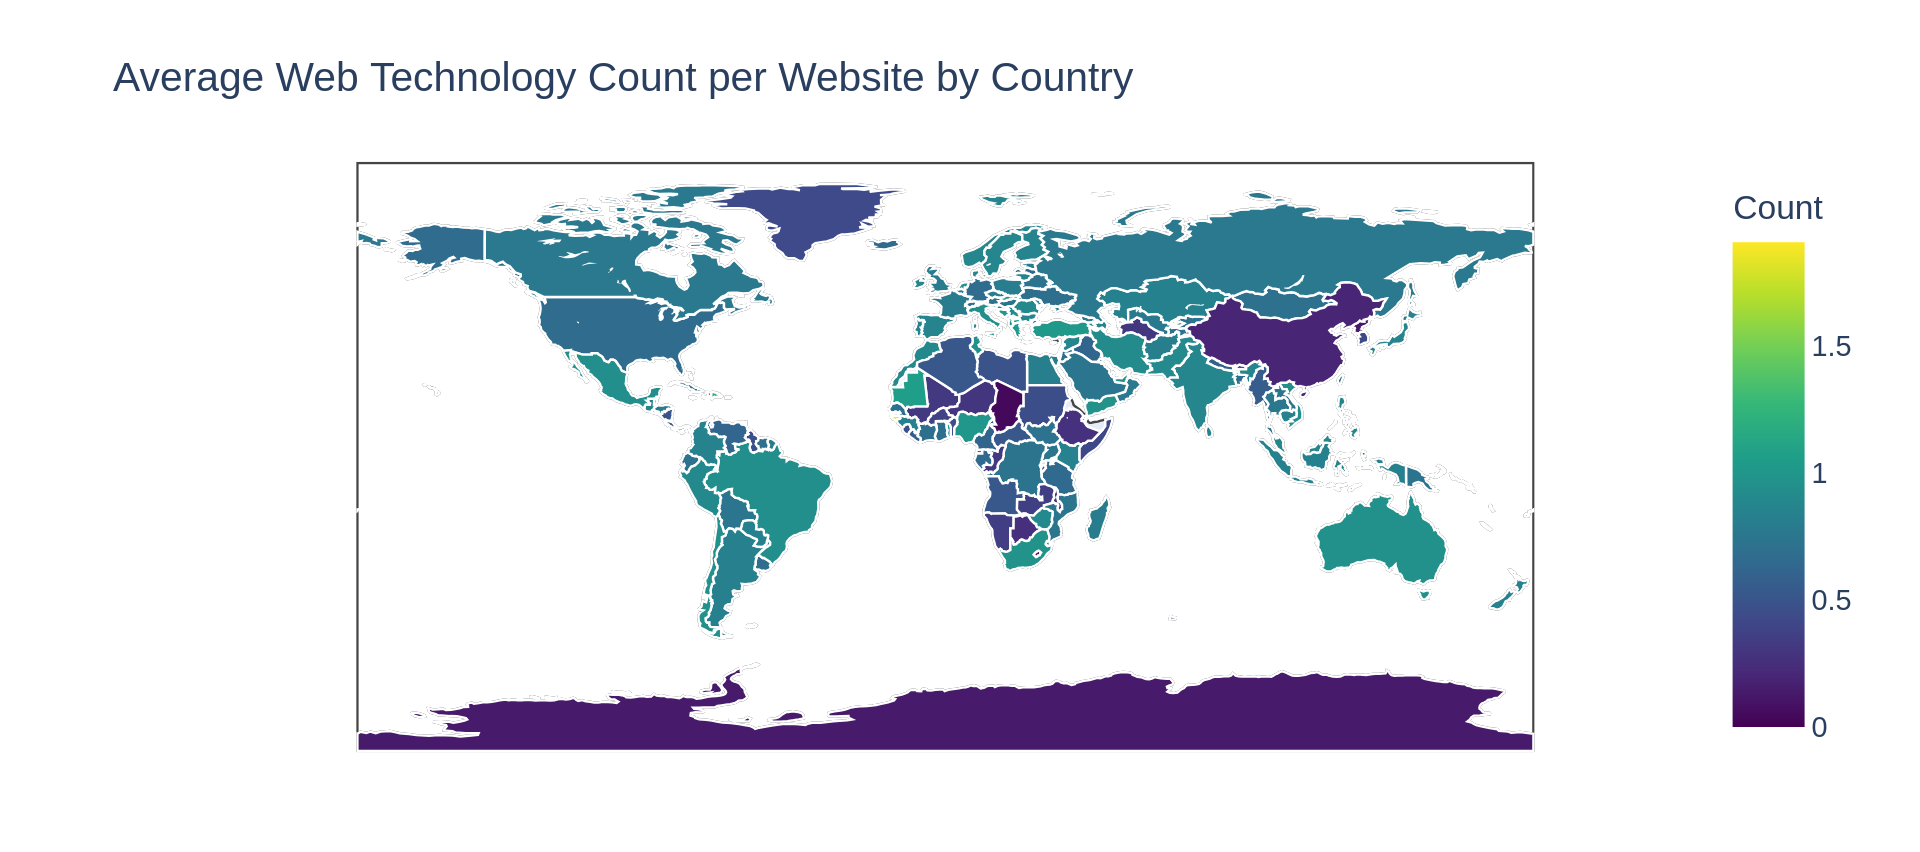
\includegraphics[width=\textwidth]{figures/charts/large/chart_fact_web_technology_choropleth_average.png}
    \caption{Average web technology count per website by country.}
    \label{fig:analysis-dataset-chart_fact_web_technology_choropleth_average}
\end{figure}

Similar to the average web technology count analysis, we can inspect the maximum web technology counts for each country, as visualized in \cref{fig:analysis-dataset-chart_fact_web_technology_choropleth_maximum}.
We keep this analysis brief for the same reason we avoided discussing countries with few attributed websites in depth: a single website with a high number of detected web technologies can make an entire country appear prominently in yellow.

For both Germany and Australia, there was at least one website with eight detected web technologies.
The maximum number of detected web technologies for Russia is seven, for China five, and for Brazil six.

\begin{figure}[H]
    \centering
    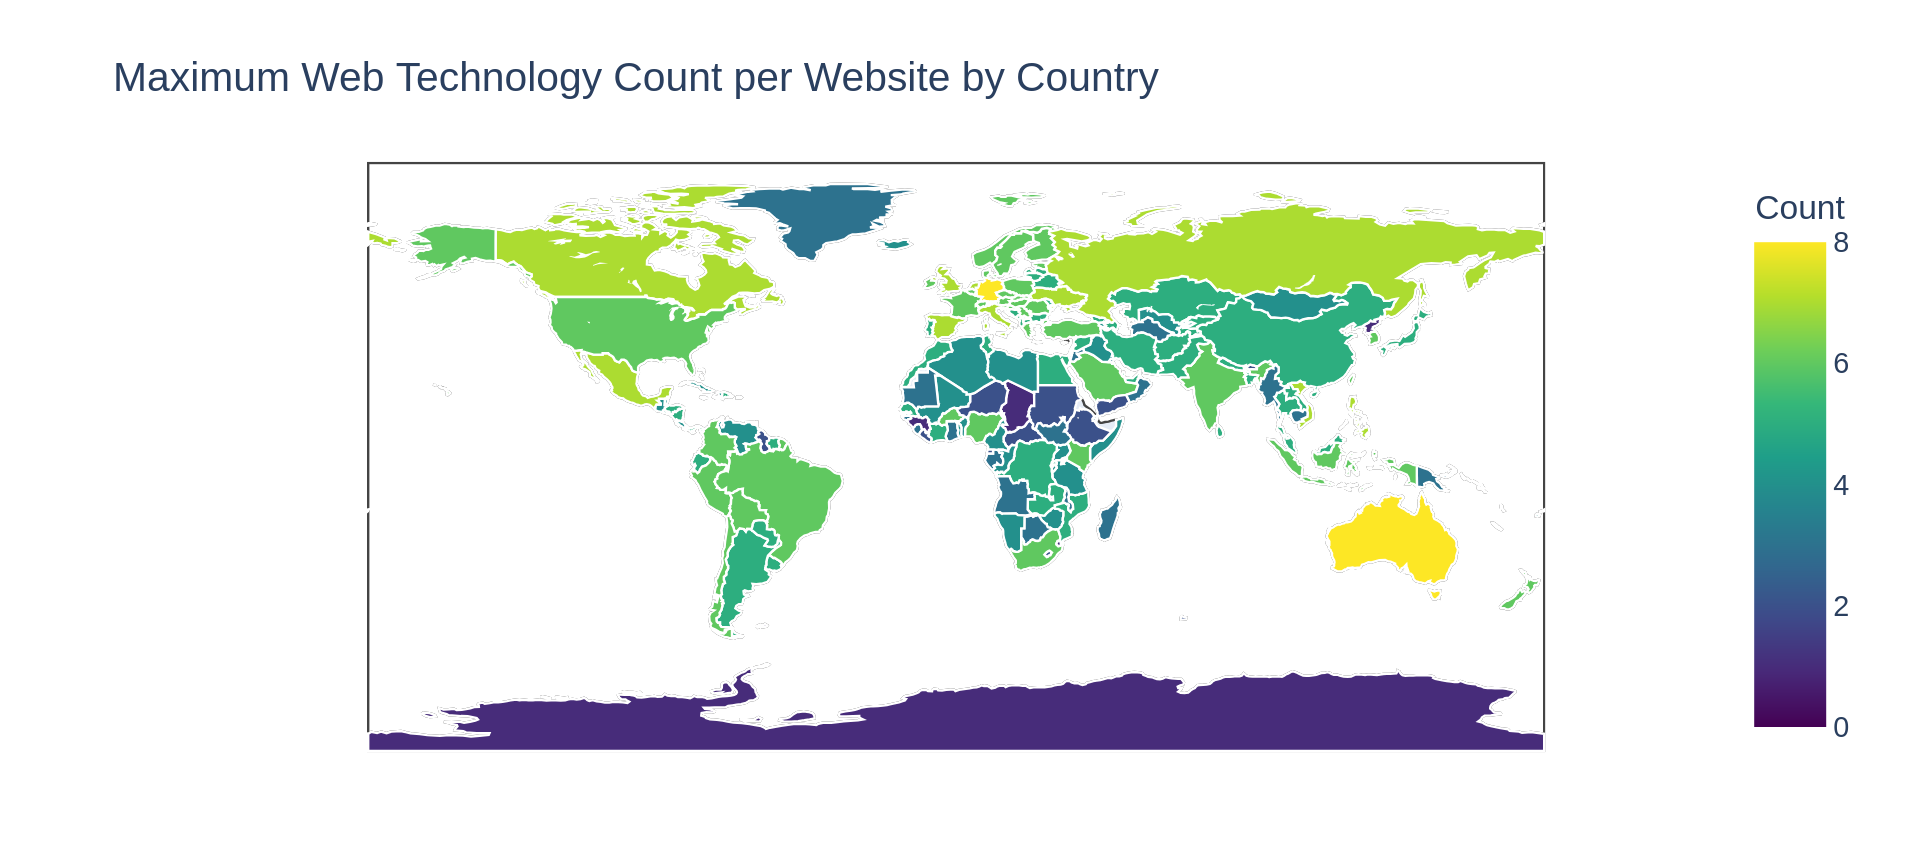
\includegraphics[width=\textwidth]{figures/charts/large/chart_fact_web_technology_choropleth_maximum.png}
    \caption{Maximum web technology count per website by country.}
    \label{fig:analysis-dataset-chart_fact_web_technology_choropleth_maximum}
\end{figure}

Whenever it seems worthwhile to explore specific differences between countries in more detail, we can generate a targeted graph using a simple function like the one shown in \cref{lst:implementation-pipeline-visualization-chart}.
\Cref{fig:analysis-dataset-chart_fact_web_technology_violin} presents a violin plot visualizing the distribution of web technology counts across web pages for the United States of America, Germany, and Japan.
The chart is normalized so that the highest web technology count equals one.

In the chart, the red area, representing Germany, extends furthest vertically at the upper end, indicating a high maximum web technology count for German websites.
At the lower end, the red area also stretches vertically, showing that many German pages have a low web technology count.
The green area, representing Japan, does not stretch as far vertically, either at the lower or upper end, suggesting fewer Japanese websites with very low or very high web technology counts compared to Germany.
However, the green area is horizontally wider in the mid-range of the y-axis, indicating that Japanese websites more commonly have a medium number of web technologies.
The blue area, representing the United States, is narrow and almost indistinguishable in the image but is more visible in the interactive \ac{html} version of the graph.
Websites from the United States follow the German pattern, with fewer websites having higher web technology counts, but overall with lower counts.

\begin{figure}[H]
    \centering
    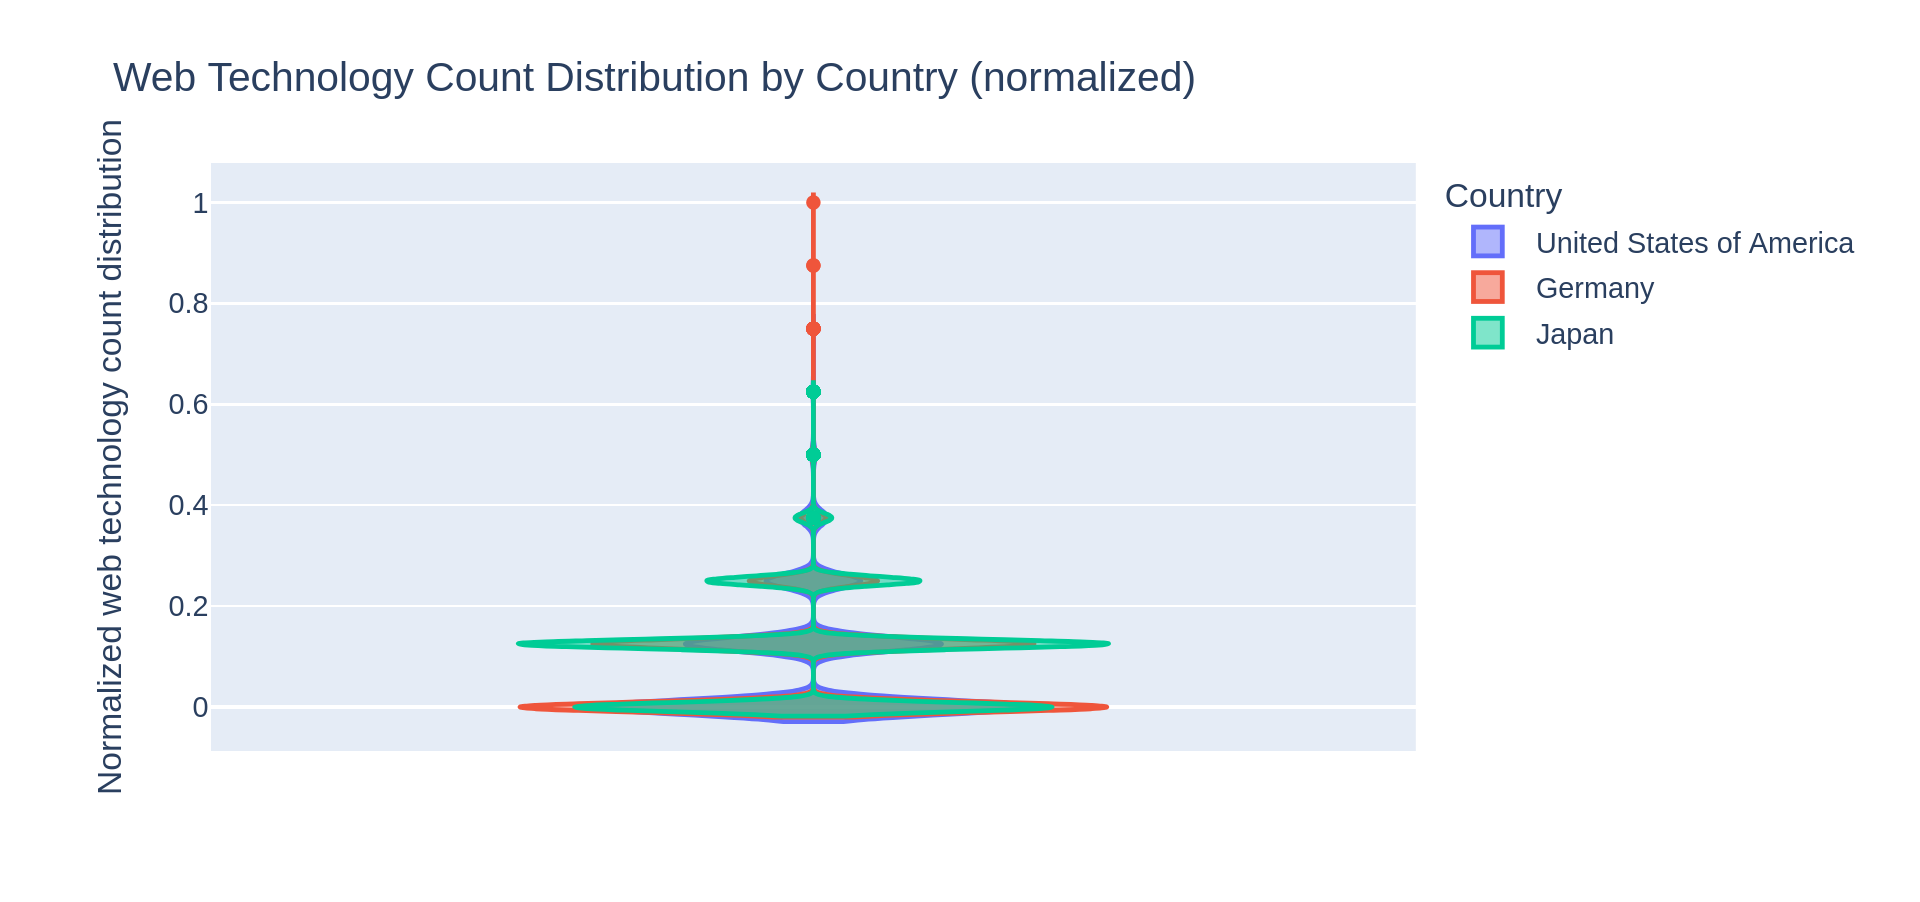
\includegraphics[width=\textwidth]{figures/charts/large/chart_fact_web_technology_violin.png}
    \caption{Distribution of web technology count by country.}
    \label{fig:analysis-dataset-chart_fact_web_technology_violin}
\end{figure}

Finally, \cref{fig:analysis-dataset-chart_fact_web_technology_heatmap_country} shows a heatmap of all web technologies across all countries.
Two main web technologies, WordPress and Google Tag Manager, are apparent due to the bright lines that span the primarily blue map.
Additionally, there is a less pronounced horizontal line with one very bright cell where Russia intersects with LiveInternet, a Russian web analytics service.
This chart highlights the importance of considering normalization for data visualization.

\Cref{fig:analysis-dataset-chart_fact_web_technology_heatmap_country_normalized} shows a version of the heatmap normalized for relative frequencies per country as well as per web technology.
In the normalized chart, many more bright cells are visible.
The alphabetical sorting of web technologies and country names results in an even distribution of highlighted fields.
Alternative sortings, such as by population, could reveal further insights.
One observation from this graph is that no single country uses the majority of web technologies, and no single web technology is used across most countries.
The majority of web technologies are embedded by only a few websites.
